\documentclass{beamer}
\usetheme{owl}           % Use metropolis theme
\newcommand\tab[1][1cm]{\hspace*{#1}}
\title{Quantifying and Mimicking Networked Behavior in Social Insects}
\date{\today}
\author{Lucas Saldyt}
\institute{Arizona State University}

\bibliographystyle{naturemag}
\begin{document}
  \maketitle
  \begin{frame}{Scope and Motivation}
      \begin{columns}
      \column{0.5\textwidth}
      \begin{itemize}
          \item Efficient Bottom-Up Self Organization (Stigmergy)
          \item Dynamic Self-Conditioned Response Behavior
          \item Generalizable Dynamics \tiny (See Applications)
      \end{itemize}
      \column{0.5\textwidth}
      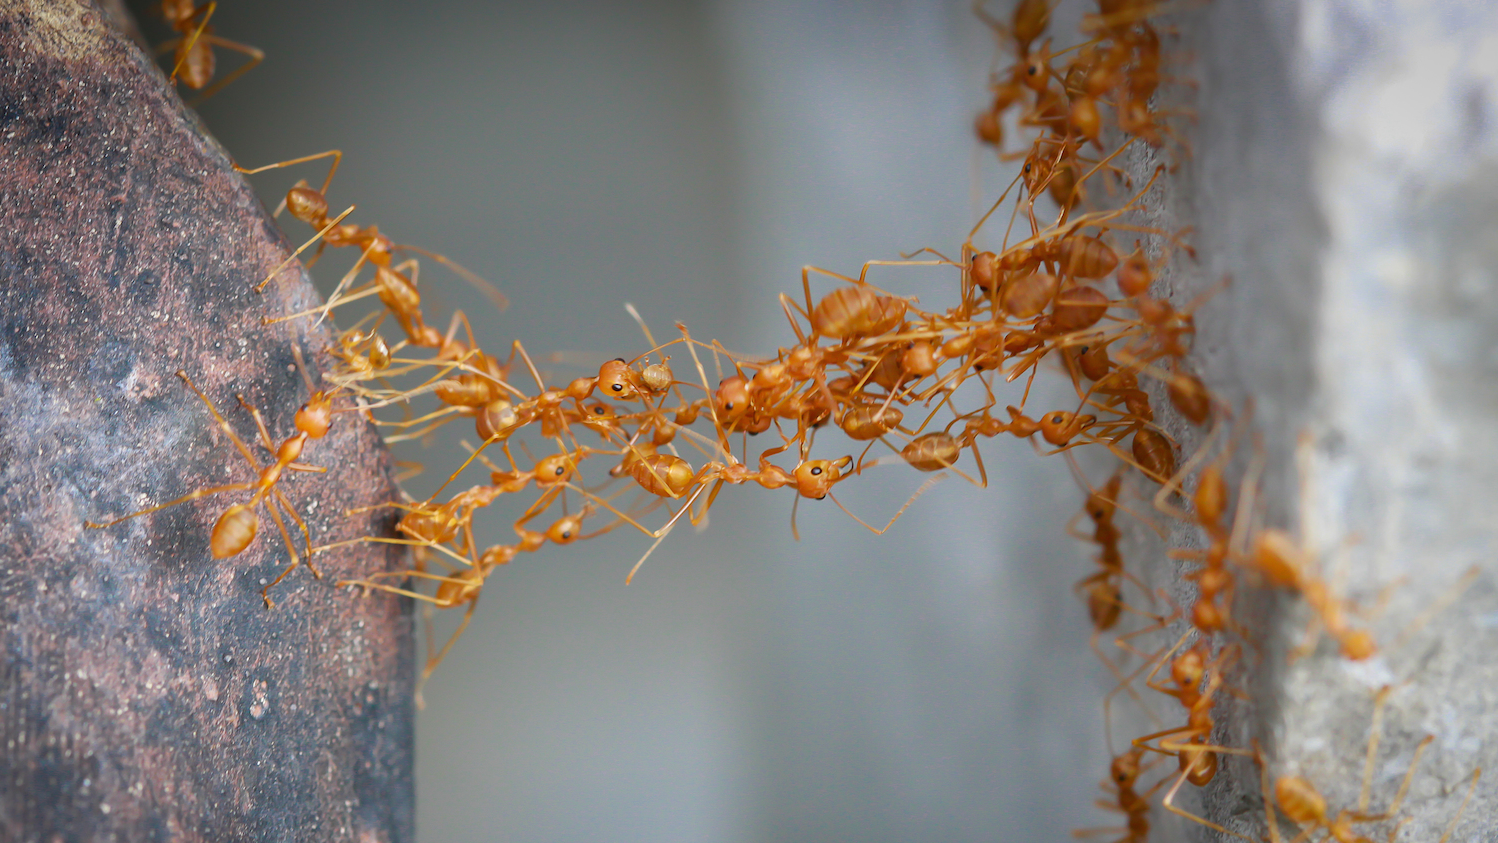
\includegraphics[scale=0.5]{ants2}
      \end{columns}
      %% lookup Guntai Ali ants
  \end{frame}

  \begin{frame}{Applications In Order of Increasing Interest}
      \begin{itemize}
          \item Behavior in other social insects
          \item Biomimetic algorithms (i.e. Pathfinding)
          \item Swarm robotics (Construction, Defense)
          \item Efficient distributed simulation
          \item Social network dynamics (Idea spread)
          \item Agent based cognitive architectures
      \end{itemize}
  \end{frame}

  \begin{frame}{Individuals}
      \begin{itemize}
          \item Solitary Insects have developed for millions of years.
          \item Individual ant brains have ~15,000 neurons. (Compare to C Elegans). \\
              \tiny (And neurons themselves are non-linear systems, so an ant colony has at least three levels of non-linearity: colony, brain, and neuron) \cite{koch_1999}. \normalsize
          \item On their own, insects are already capable of non-trivial tasks (like pathfinding)
      \end{itemize}
  \end{frame}

  \begin{frame}{Eusociality}
      \begin{itemize}
          \item Insects fill separate roles with a high degree of cooperation \normalsize \cite{gelblum2015ant}
          \item Colony-level behavior comes from communication. Ants use pheromone systems and touch-communication in social networks. \cite{fewell_2003}
              \begin{itemize}
                  \item Actions range from individual to collective (with substates inbetween) \cite{feinerman2017individual}. \tiny (See Collective Cognition Slide) \normalsize
              \end{itemize}
          \item High connectivity (possibility for rapid spreading) \cite{gernat2018automated}
          \item Self-regulation \cite{heyman2017ants}
          \item Social
          \item ``Stigmergy`` (Next Slide) \cite{fonio2016locally}
      \end{itemize}
  \end{frame}

  \begin{frame}{Stigmergy}
      ``Stigmergy is a form of self-organization social network. It produces complex, seemingly intelligent structures, without need for any planning, control, or even direct communication between the agents. As such it supports efficient collaboration between extremely simple agents, who lack any memory, intelligence or even individual awareness of each other`` \\ \tab - Wikipedia (Itself a stigmergic system!)
  \end{frame} 

  \begin{frame}{Collective Cognition}
      \begin{itemize}
          \item Signals like alarm unconditioned. \tiny (~Centralized?) \normalsize
          \item Signals like trail finding double-checked \tiny (Escape local minima!) \normalsize
          \item Stigmergic Construction of particular interest:
              \begin{itemize}
                  \item Building blocks initially placed ``randomly``, and infused with pheromones.
                  \item Secondary blocks placed based on other blocks and recency
                  \item Local rules become intricate nests
                  \item More of a distributed behavior than a centralized one.
              \end{itemize}
      \end{itemize}
  \end{frame}

  \begin{frame}{Networks}
      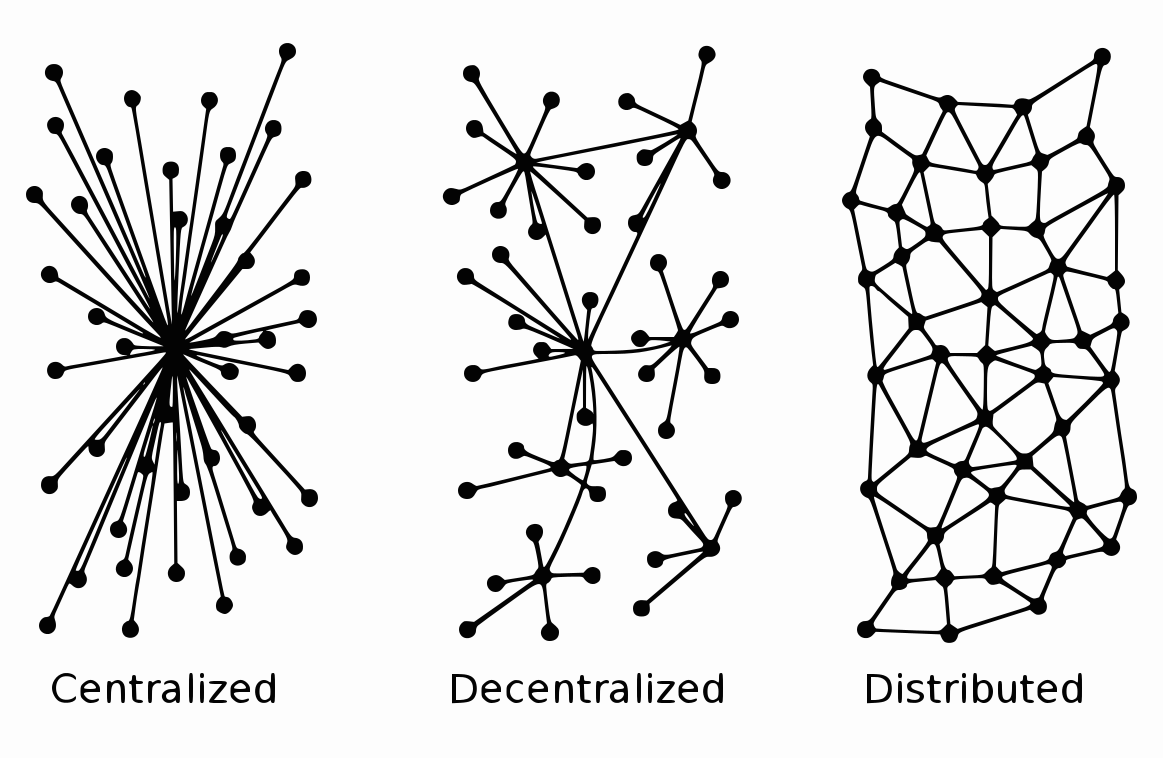
\includegraphics[scale=0.25]{networks}
  \end{frame}
  \begin{frame}{Networks 2}
      \begin{itemize}
          \item We can quantify the degree of centrality, decentrality, or distribution of a network at each time step.
          \item Certain tasks will cause different networked behavior.
          \item For example, alarm response is between centralized and decentralized behavior, much like disease spreading.
          \item Networks may have general properties observable in other systems \cite{sporns_2004, watts_strogatz_2011}.
          \item Weighted clustering coefficient:
              \[
                  C_{\omega} = \frac{\sum_{\tau \Delta}^{} \omega}{\sum_{\tau}^{} \omega}
              \] \newline
              Using different weights, clustering coefficient can quantify several things. Inter-ant distance as weight gives primary results.
      \end{itemize}
  \end{frame}

  \begin{frame}{Ant Model}
      Simple model: random correlated walk, where proximity determines spreading activation.
      \begin{itemize}
          \item Individual paths/locations wont be maintained
          \item Are group statistics maintained? (Like clustering coefficient or average velocity)
      \end{itemize}
  \end{frame}

  \begin{frame}{Experiments}
      This project focuses on the temporal network of ants.
      Ants are observed by a 30hz camera (discretely).
      At each timestep, we know the network of ants. 
      We model this as a graph, with edges drawn as euclidean distances between each ant.
      %% While it is extremely difficult to create a model that maintains ant location and velocity, we hope to create a model that can produce the same network metrics and averaged behavior.
      Given the graph, we can calculate, for example, the way that the clustering coefficient changes over time\cite{saramaki2007generalizations}.
      This indicates distribution or centrality, and can be compared to our computer model.
  \end{frame}

  \begin{frame}{Cognitive Architectures}
      \begin{itemize}
          \item First cognitive architecture in the 50s (Newell and Simon). Turned into SOAR.
          \item Copycat: agent based model of creative problem solving
          \item LIDA: Combined general cognitive psychology and SOAR with Copycat architecture.
          \item Agent based approaches like copycat or lida are comparable to an agent based ant model.
          \item Both also are controlled by PDE.
          \item For instance, copycat has equillibrium points and attractors -- some of them intentionally built in.
      \end{itemize}
  \end{frame}

  \begin{frame}{LIDA}
      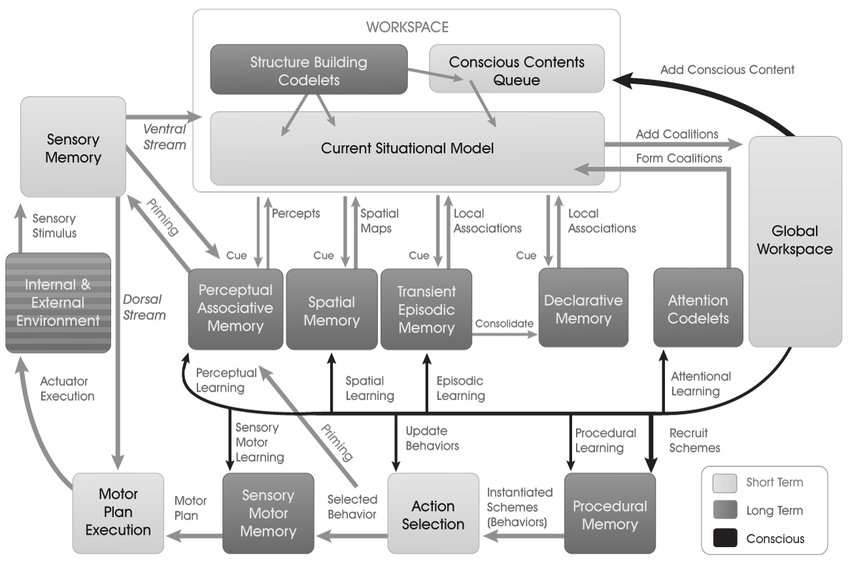
\includegraphics[scale=0.3333]{lida}
  \end{frame}

  \begin{frame}{Bibliography}
      \bibliography{sources/insects,sources/brains,sources/ant_system,sources/networks,sources/misc}
  \end{frame}

\end{document}
